\section{Flipping Edges}
\label{sect:flipping-edges}

Let us now discuss the edge flip mentioned in the previous sections.
An internal edge $\{u,v\}$ is incident to two different internal faces $f$, $g$.
Let $x$ and $y$ denote the third vertex bounding $f$ and $g$, respectively.
It is $x \neq y$ because the cluster graph is simple.
Flipping the edge $\{u,v\}$ would replace it with the edge $\{x,y\}$.
Consequently, this operation is only permitted iff $x$ and $y$ are not already adjacent \emdash{} otherwise, we would introduce a duplicate adjacency.
\Cref{fig:flip-edge-example-internal} shows an example of a valid edge flip operation.

\begin{figure}[H]
	\centering
	\subfigure[]{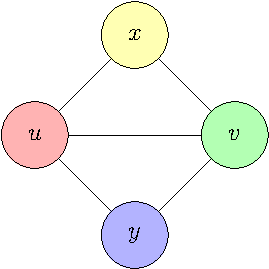
\includegraphics[height=29mm]{Resources/FlipEdge-Example-Internal-1.pdf}}
	\quad
	\subfigure[]{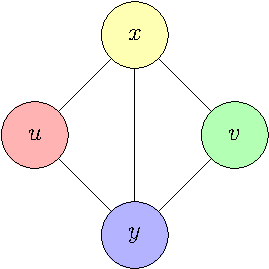
\includegraphics[height=29mm]{Resources/FlipEdge-Example-Internal-2.pdf}}
	\qquad
	\subfigure[]{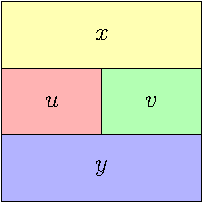
\includegraphics[height=29mm]{Resources/FlipEdge-Example-Internal-3.pdf}}
	\quad
	\subfigure[]{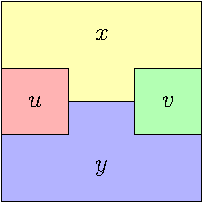
\includegraphics[height=29mm]{Resources/FlipEdge-Example-Internal-4.pdf}}
	\caption{A cluster graph and a polygonal dual thereof, before (a, c) and after (b, d) flipping the internal edge $\{u,v\}$.}
	\label{fig:flip-edge-example-internal}
\end{figure}

An edge flip in a cluster graph translates to region adjacencies being flipped in its dual.
Given a polygonal dual of some cluster graph, we apply an edge flip in two phases.
First, we contract the region boundary we want to remove into a single point, creating a degenerate contact representation in which four regions meet in a point.
In the second phase, we create a region boundary in the opposite direction, getting rid of the degeneracy at the point into which the original boundary has been contracted.

Let $u$ and $v$ be two adjacent faces in the polygonal dual whose boundary we want to contract.
Also, let path $P_{uv}$ be the maximal common boundary between $u$ and $v$, oriented such that $u$ lies on the left of it, and $v$ lies on the right of it.
At both endpoints of the path, $u$ and $v$ meet with a third face.
We denote the third face incident to the path's first vertex by $x$ and the third face incident to the path's last vertex by $y$, as illustrated in \cref{fig:flip-edge-example-internal}.
To contract the $u$-$v$-boundary into a single point, we repeatedly contract a peripheral edge on the boundary until the last edge has been contracted.
We do so on alternating ends, \ie{}, we start by contracting the first edge, then the last, then the first again, etc.

\begin{figure}[H]
	\centering
	\subfigure[]{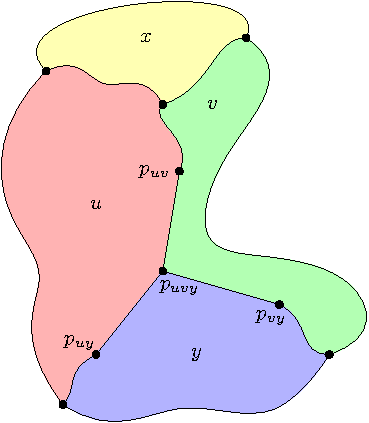
\includegraphics[width=40mm]{Resources/FlipEdge-ContractBoundaryBelow-1.pdf}\label{subfig:flip-edge-contract-boundary-below-1}}
	\quad
	\subfigure[]{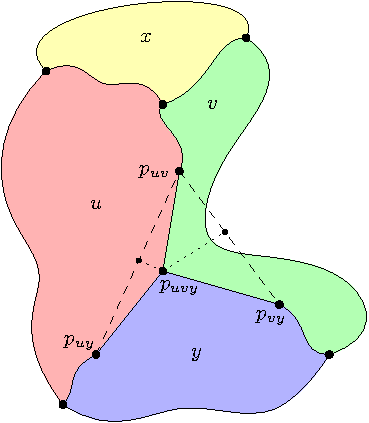
\includegraphics[width=40mm]{Resources/FlipEdge-ContractBoundaryBelow-2.pdf}\label{subfig:flip-edge-contract-boundary-below-2}}
	\quad
	\subfigure[]{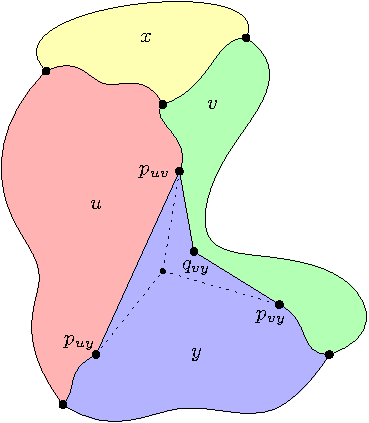
\includegraphics[width=40mm]{Resources/FlipEdge-ContractBoundaryBelow-3.pdf}\label{subfig:flip-edge-contract-boundary-below-3}}
	\caption{A contact representation before (a) and after (c) contracting the peripheral edge $\{p_{uv},p_{uvy}\}$ on the $u$-$v$-boundary away from $y$. (b) shows the construction of potential subdivision vertices.}
	\label{fig:flip-edge-contract-boundary-below}
\end{figure}

\Cref{fig:flip-edge-contract-boundary-below} illustrates how we contract the first edge of the oriented upwards without introducing edge crossings.
We describe only this construction in writing; the contraction of the last edge works virtually the same way and is illustrated in \cref{fig:flip-edge-contract-boundary-above}.
Let $p_{uvy}$ denote the vertex where the faces $u$, $v$, and $y$ meet and $p_{uy}$ and $p_{vy}$ the subdivision vertices on the $u$-$y$- and $v$-$y$-boundaries that are incident to $p_{uvy}$, respectively.
If the $u$-$y$- or $v$-$y$-boundary consists of only one edge, we subdivide it at its midpoint first.
Let $p_{uv}$ be the subdivision vertex on the $u$-$v$-boundary that is incident to $p_{uvy}$ or the last vertex of the oriented boundary if no such subdivision vertex exists.
To reduce the length of the $u$-$v$-boundary by one, we would want to remove $p_{uvy}$ and its incident edges and add edges from $p_{uv}$ to both $p_{uy}$ and $p_{vy}$.
These edges may introduce crossings, though, as illustrated by the dashed lines in \cref{subfig:flip-edge-contract-boundary-above-2} and \cref{subfig:flip-edge-contract-boundary-below-2}.
However, with just one bend on each of the edges, we can guarantee that no edge crossings are created:

\begin{itemize}
\item If adding the edge between $p_{uv}$ and $p_{ay}$ ($a \in \{u,v\}$) does not introduce a crossing, we simply add the edge.
(for $a = u$ in \cref{subfig:flip-edge-contract-boundary-below-2})
\item Otherwise, if the internal angle of face $a$ at $p_{uvy}$ is $180^\circ$ or more, we place the bend at $p_{uvy}$, \ie{}, we insert the edge $\{p_{uv},p_{ay}\}$ and subdivide it with a new vertex $q_{ay}$ at the position of $p_{uvy}$.
Note that at most one of the faces can have an internal angle at $p_{uvy}$ that is $180^\circ$ or more.
(for $a = v$ in \cref{subfig:flip-edge-contract-boundary-above-2})
\item Otherwise, we search for a bend location in the form of a subdivision vertex $q_{ay}$ somewhere on the outward-pointing bisector of the angle $\angle_{p_{ay}p_{uvy}p_{uv}}$ (dotted lines in \cref{subfig:flip-edge-contract-boundary-below-2} and \cref{subfig:flip-edge-contract-boundary-above-2}).
We start looking at the point where the bisector intersects the segment from $p_{uv}$ to $p_{ay}$ and repeatedly divide the remaining distance to $p_{uvy}$ in half until we find a bend location for which the bent edge from $p_{uv}$ to $p_{ay}$ would not introduce edge crossings.
As the candidate location moves infinitesimally close to $p_{uvy}$, we are guaranteed to find one that does not introduce crossings.
(for $a = v$ in \cref{subfig:flip-edge-contract-boundary-below-3} and $a = u$ in \cref{subfig:flip-edge-contract-boundary-above-3})
\end{itemize}

\begin{figure}[H]
	\centering
	\subfigure[]{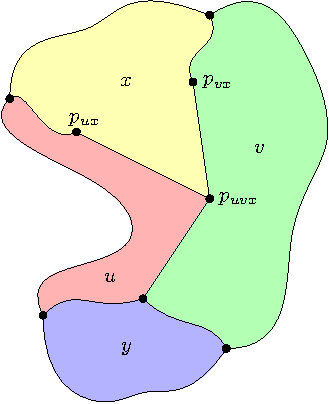
\includegraphics[width=40mm]{Resources/FlipEdge-ContractBoundaryAbove-1.pdf}\label{subfig:flip-edge-contract-boundary-above-1}}
	\quad
	\subfigure[]{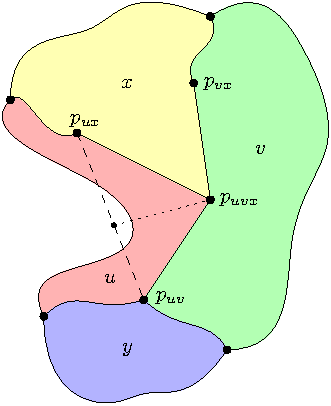
\includegraphics[width=40mm]{Resources/FlipEdge-ContractBoundaryAbove-2.pdf}\label{subfig:flip-edge-contract-boundary-above-2}}
	\quad
	\subfigure[]{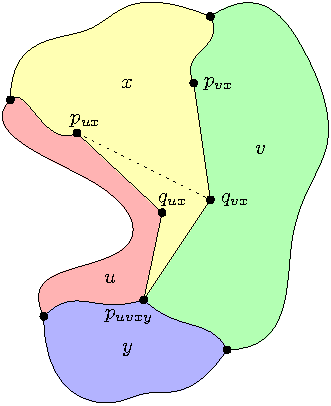
\includegraphics[width=40mm]{Resources/FlipEdge-ContractBoundaryAbove-3.pdf}\label{subfig:flip-edge-contract-boundary-above-3}}
	\caption{A contact representation before (a) and after (c) contracting the last remaining edge $\{p_{uvx},p_{uvy}\}$ on the $u$-$v$-boundary away from $y$. (b) shows the construction of potential subdivision vertices.}
	\label{fig:flip-edge-contract-boundary-above}
\end{figure}

Once the $u$-$v$-boundary has been contracted into a single vertex $p_{uvxy}$ where all four faces $u$, $v$, $x$, and $y$ now meet, as shown in \cref{subfig:flip-edge-contract-boundary-above-3}, we need to resolve the degeneracy and create a boundary in the opposite direction, \ie{}, an $x$-$y$-boundary.
Let $p_{ux}$, $p_{uy}$, $p_{vx}$, and $p_{vy}$ denote the subdivision vertices on the respective boundaries that are incident to $p_{uvxy}$.
Again, if a boundary consists of only one edge, we subdivide it at its midpoint first such that all $p_{ab}$ exist.
We are now looking to stretch the vertex $p_{uvxy}$ back into a non-degenerate $x$-$y$-boundary, as illustrated in \cref{fig:flip-edge-create-boundary}.
Analogous to above, we search for a position in face $u$ ($v$) where we can place a vertex $q_u$ ($q_v$) and add edges to $p_{uvxy}$, $p_{ux}$, and $p_{uy}$ ($p_{uvxy}$, $p_{vx}$, and $p_{vy}$) without introducing crossings.
We start at the intersection of the segment between $p_{ux}$ and $p_{uy}$ (between $p_{vx}$ and $p_{vy}$) and the bisector of $\angle_{p_{ux}p_{uvxy}p_{uy}}$ ($\angle_{p_{vx}p_{uvxy}p_{vy}}$) and repeatedly divide the distance to $p_{uvxy}$ in half until we find a valid position.
Once we have found such a position, we insert the vertex $q_u$ ($q_v$) along with the aforementioned edges and remove the edges $\{p_{uvxy},p_{ux}\}$ and $\{p_{uvxy},p_{uy}\}$ ($\{p_{uvxy},p_{vx}\}$ and $\{p_{uvxy},p_{vy}\}$).
In case $\measuredangle_{p_{ux}p_{uvxy}p_{uy}} \geq 180^\circ$ ($\measuredangle_{p_{vx}p_{uvxy}p_{vy}} \geq 180^\circ$), we will not find such a position and shall not make an adjustment on that side.
However, again, this event cannot occur for both $u$ and $v$ at the same time.
As a result, we always create an $x$-$y$-boundary that consists of at least one edge.

\begin{figure}[H]
	\centering
	\subfigure[]{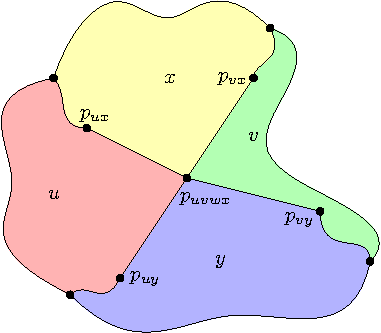
\includegraphics[width=45mm]{Resources/FlipEdge-StretchBoundary-1.pdf}}
	\quad
	\subfigure[]{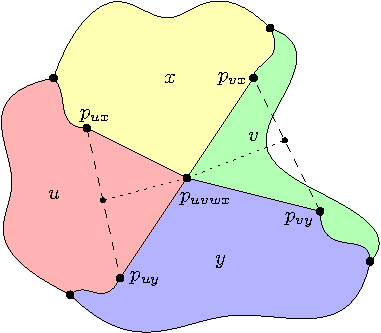
\includegraphics[width=45mm]{Resources/FlipEdge-StretchBoundary-2.pdf}}
	\quad
	\subfigure[]{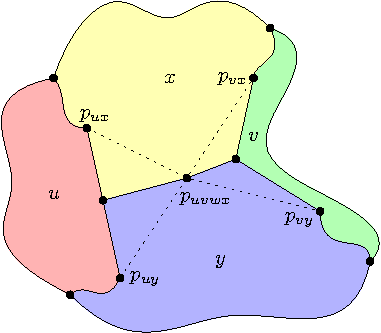
\includegraphics[width=45mm]{Resources/FlipEdge-StretchBoundary-3.pdf}}
	\caption{A contact representation before (a) and after (c) creating a non-degenerate yellow-blue adjacency. (b) shows the construction of potential subdivision vertices.}
	\label{fig:flip-edge-create-boundary}
\end{figure}



\paragraph{Inserting and Removing Edges}

As clusters in our data set grow increasingly similar, we may want to indicate this similarity with new edges between existing clusters in the cluster graph.
Similarly, clusters can grow apart, and we may want to remove edges between clusters in the cluster graph.
However, because the filtered cluster graph is internally triangulated, we cannot insert any more edges on the inside of the graph.
Removing an internal edge is not permitted either, as that would create a hole in the graph.
Consequently, we can insert edges only in the outer face and remove edges only on the outer face.

On top of that, inserting an edge in the outer face is only possible if it preserves the cluster graph's internal triangulatedness.
Therefore, inserting an edge $\{u,w\}$ is only permitted iff $u$ and $w$ lie on the outer face and have a neighbor $v$ in common that also lies on the outer face.
The inserted edge is then embedded such that it forms a new triangular internal face with $v$ and turns $v$ into an internal vertex.
If exactly four vertices bound the outer face before inserting the edge $\{u,w\}$, there exist two candidates for $v$.
In this case, it must be made explicit which one is supposed to become internal and which one is supposed to remain on the outer face.
\Cref{fig:flip-edge-example-insert} shows an example of a valid edge insertion.

\begin{figure}[H]
	\centering
	\subfigure[]{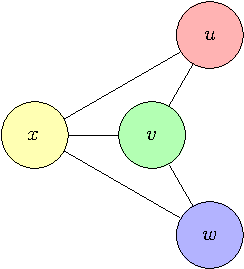
\includegraphics[height=29mm]{Resources/FlipEdge-Example-Insert-1.pdf}}
	\quad
	\subfigure[]{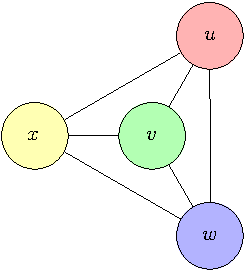
\includegraphics[height=29mm]{Resources/FlipEdge-Example-Insert-2.pdf}}
	\qquad
	\subfigure[]{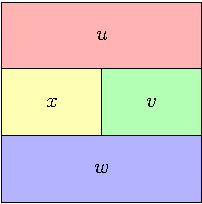
\includegraphics[height=29mm]{Resources/FlipEdge-Example-Insert-3.pdf}}
	\quad
	\subfigure[]{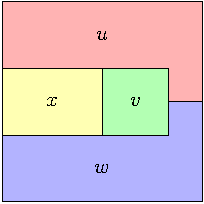
\includegraphics[height=29mm]{Resources/FlipEdge-Example-Insert-4.pdf}}
	\caption{A cluster graph and a polygonal dual thereof, before (a, c) and after (b, d) inserting the edge $\{u,w\}$ to form an internal triangular face with $v$.}
	\label{fig:flip-edge-example-insert}
\end{figure}

Removing an edge $\{u,w\}$ on the outer face of the cluster graph is only permitted if the graph remains biconnected.
This property is preserved iff both $u$ and $w$ have degree $d(\cdot) \geq 3$ and the third vertex $v$ in the internal face bounded by $\{u,w\}$ does not already lie on the outer face.
If that vertex laid on the outer face already, we would end up creating a duplicate adjacency/boundary between $v$ and the outer face, which we specifically excluded in \cref{chap:preliminaries}.
\Cref{fig:flip-edge-example-remove} shows an example of a valid edge removal.

\begin{figure}[H]
	\centering
	\subfigure[]{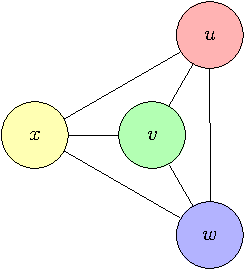
\includegraphics[height=29mm]{Resources/FlipEdge-Example-Remove-1.pdf}}
	\quad
	\subfigure[]{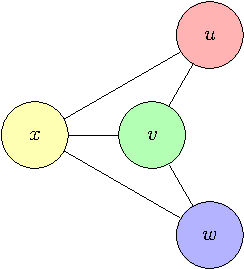
\includegraphics[height=29mm]{Resources/FlipEdge-Example-Remove-2.pdf}}
	\qquad
	\subfigure[]{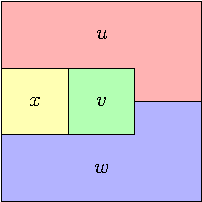
\includegraphics[height=29mm]{Resources/FlipEdge-Example-Remove-3.pdf}}
	\quad
	\subfigure[]{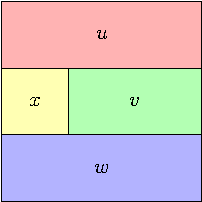
\includegraphics[height=29mm]{Resources/FlipEdge-Example-Remove-4.pdf}}
	\caption{A cluster graph and a polygonal dual thereof, before (a, c) and after (b, d) removing the edge $\{u,w\}$.}
	\label{fig:flip-edge-example-remove}
\end{figure}

Both of these operations are again a special case of the generic edge flip discussed above with a quirk:
Instead of four internal faces, they involve three internal faces and the implicit outer face.

In the example from \cref{fig:flip-edge-example-insert}, we make $v$ into an internal vertex by inserting the edge $\{u,w\}$, removing $v$'s boundary with the outer face in the dual and creating a $u$-$w$-boundary in turn.
Again, recall that in the construction of the augmented dual from \cref{def:augmented-dual}, we insert a helper vertex $v^+$ in the outer face and add edges to all vertices on the original outer face.
This helper vertex and its adjacencies correspond to the outer face and its boundaries in the dual.
When inserting an edge in the outer face, we are essentially flipping the helper edge $\{v,v^+\}$ to become the inserted edge $\{u,w\}$.
Therefore, we apply the same procedure as discussed for the edge flip above, contracting the boundary between $v$ and the outer face into a single point and then creating a non-degenerate $u$-$w$-boundary.

Similarly, when removing an edge $\{u,w\}$ on the outer face as in \cref{fig:flip-edge-example-remove}, a previously-internal vertex $v$ moves onto the outer face.
We can think of it as flipping the edge to be removed to become the helper edge $\{v,v^+\}$.
In the polygonal dual, this gets rid of the $u$-$w$-boundary and creates a boundary between $v$ and the implicit outer face in turn.
Again, we apply the same procedure as discussed for the edge flip, first contracting the $u$-$w$-boundary into a single point and then creating a non-degenerate boundary between $v$ and the outer face.
